\section{Основные этапы выполнения}
Для выполнения первого задания были созданы абстрактные классы \texttt{Parser} и \texttt{Presenter}.
Далее от них были унаследованы и реализованы классы \texttt{XMLDefaultParser} и \texttt{YAMLDefaultPresenter}.
Парсинг реализован с помощью поиска необходимых тегов в тексте самым тривиальным способом.

Для выполнения первого дополнительного задания были созданы новые классы \texttt{XMLParser} и \texttt{YAMLPresenter} с помощью
библиотек \texttt{xml.etree.ElementTree} и \texttt{pyyaml} соответственно.
Различий в работе парсеров нет, различия в работе между \texttt{YAMLDefaultPresenter} и \texttt{YAMLPresenter} заключаются лишь
в отступах.

Для выполнения второго лабораторного задания был создан класс \texttt{XMLRegexParser}.
Алгоритм остался таким же, как и в первом задании, но поиск выполнен с помощью регулярных выражений.

Для выполнения третьего дополнительного задания были использованы библиотеки \texttt{matplotlib} и \texttt{multiprocessing
}для начертания графика и более быстрого теста производительности парсеров. На рисунке~\ref{fig:all} представлены все парсеры,
на рисунке~\ref{fig:fastest} представлены парсер на регулярных выражениях и с помощью библиотеки.
На рисунке~\ref{fig:presenters} представлено сравнение презентеров.

\begin{figure}[ht]
    \centering
    \begin{subfigure}[b]{0.45\textwidth}
        \centering
        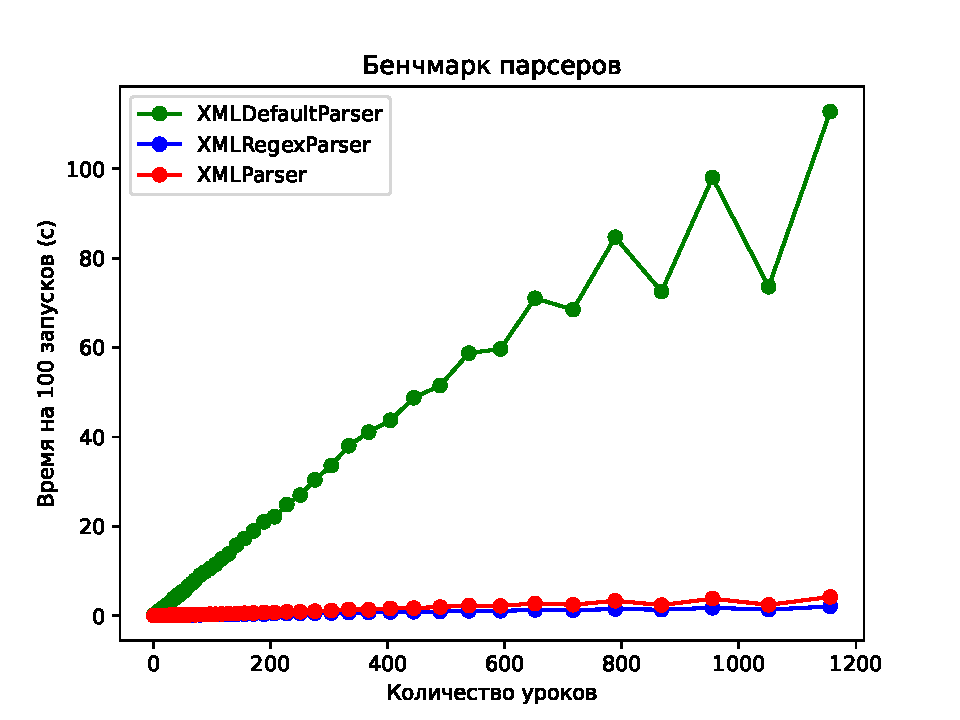
\includegraphics[width=\textwidth]{img/benchmark_all.pdf}
        \caption{Сравнение всех парсеров}
        \label{fig:all}
    \end{subfigure}
    \begin{subfigure}[b]{0.45\textwidth}
        \centering
        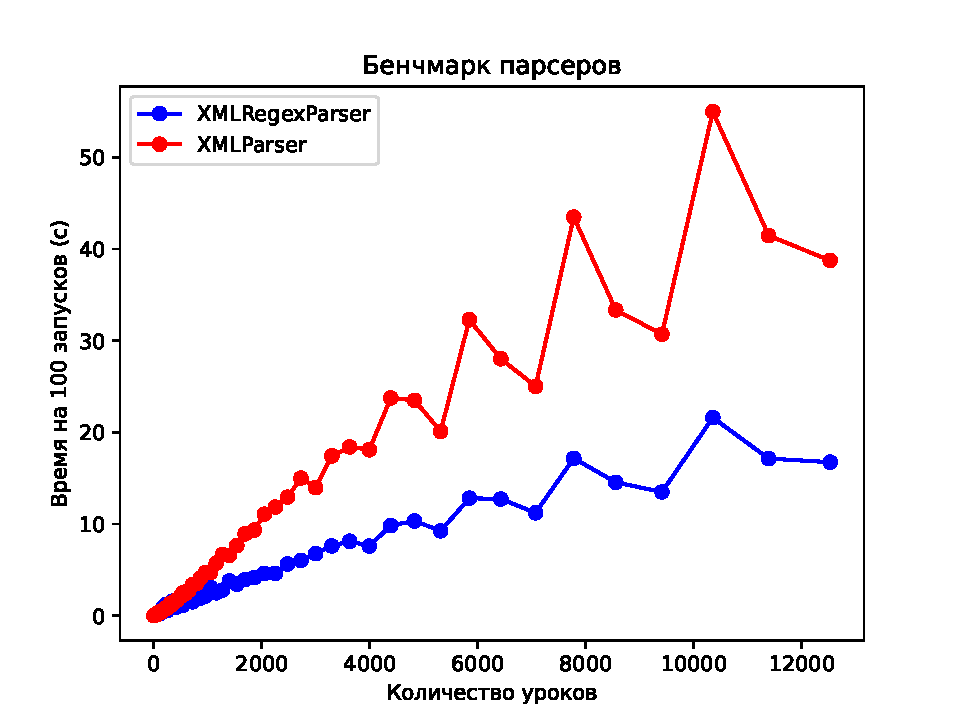
\includegraphics[width=\textwidth]{img/benchmark_fastest.pdf}
        \caption{Сравнение самых быстрых парсеров}
        \label{fig:fastest}
    \end{subfigure}
    \caption{Сравнение парсеров}
\end{figure}

\begin{figure}[ht]
    \centering
    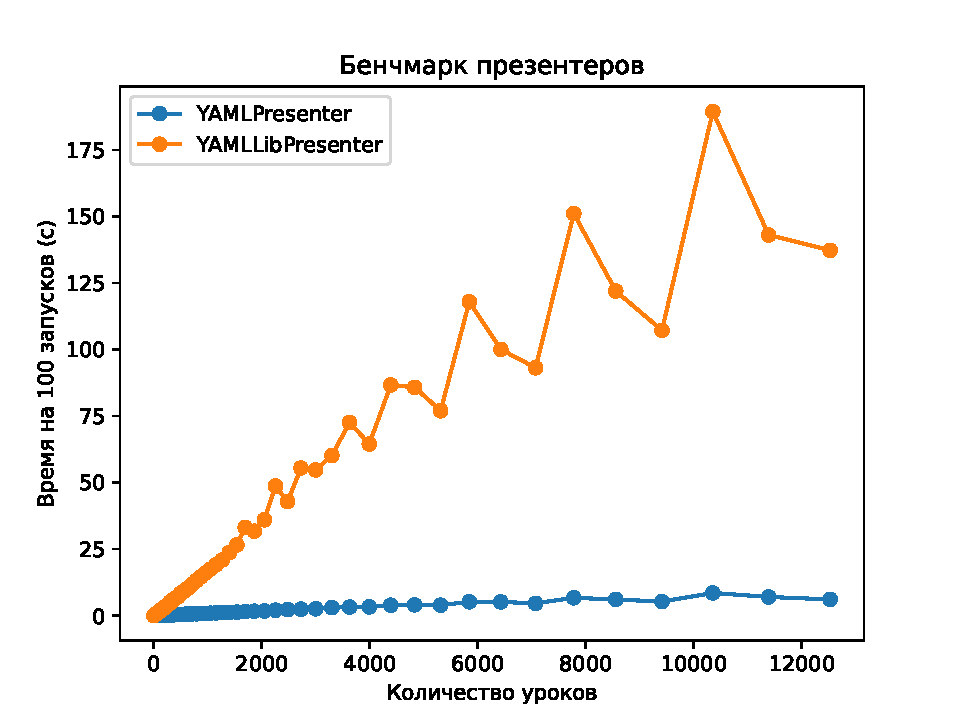
\includegraphics[width=0.45\textwidth]{img/benchmark_p.pdf}
    \caption{Сравнение презентеров}
    \label{fig:presenters}
\end{figure}

Слишком медленная работа XMLDefaultParser объясняется неэффективным алгоритмом нахождения подстроки в строке за $O(n^2)$.
Более быстрая работа \texttt{XMLRegexParser} по сравнению с \texttt{XMLParser} объясняется тем, что \texttt{XMLParser} полностью строит синтаксическое дерево
и проверяет его корректность и лишь затем достает необходимые теги. \texttt{XMLRegexParser} просто ищет нужные теги среди других тегов.

Более медленная работа \texttt{YAMLLibPresenter} объясняется переводом сначала в объект типа \texttt{dict}, и лишь затем переводом в формат YAML.
Для работы \texttt{YAMLPresenter} этого не нужно.

Для выполнения четвертого задания был выбран формат \texttt{protobuf} и были написаны классы \texttt{ProtobufPresenter} и \texttt{ProtobufParser}.
Описание структур данных содержится в файле \texttt{schedule} \texttt{/schedule.proto}

\section{Исходный код}
Исходный код программы доступен в git-репозитории по ссылке \url{https://github.com/FEgor04/labs/tree/main/informatics/lab4}